\documentclass[a4paper,12pt]{article}
\usepackage[french]{babel}
\usepackage{graphicx}
\graphicspath{{figures/}}
\usepackage{array}
\usepackage{listings}
\usepackage{amsmath}
\usepackage{multicol}%plusierus colones
\usepackage{multirow}
\usepackage{fancyheadings} %%%%logo
\renewcommand{\baselinestretch}{1.5}%%%%interligne
\usepackage{fancyhdr} %%%%%%en-tête
\usepackage[utf8]{inputenc}%%%%utp-8 accents
\usepackage{multirow}
\usepackage{listings}
\pagestyle{fancy} %: Numérotation des pages.
\lhead{Sven Borden et Eric Brunner}% :	On personnalisera cette en-tête. haut de page gauche
\chead{2M03} %: On personnalisera cette en-tête. haut de page centre
\rhead{\today} %: On personnalisera cette en-tête. haut de page droite
\lfoot{Travail de Maturité} %:	On personnalisera cette en-tête. pied de page gauche
\cfoot{\textbf{Page \thepage/\pageref{LastPage}}} %: On personnalisera cette en-tête. pied de page centre
\rfoot{Robotique} %: On personnalisera cette en-tête. pied de page droite
\renewcommand{\headrulewidth}{0.4pt} % Trace un trait de séparation de largeur 0,4 point. Mettre 0pt pour supprimer le trait.
\renewcommand{\footrulewidth}{0.4pt} %: Trace un trait de séparation de largeur 0,4 point. Mettre 0pt pour supprimer le trait.
\usepackage{lastpage} %%%% conteur de page, ( 1/3 ,2/3...)
\usepackage{ucs}%%%peut être pour la fraction continue
\setlength{\hoffset}{-18pt}         
\setlength{\oddsidemargin}{2.5cm} % Marge gauche sur pages impaires
\setlength{\evensidemargin}{2.5cm} % Marge gauche sur pages paires
\setlength{\marginparwidth}{0pt} % Largeur de note dans la marge
\setlength{\textwidth}{13.3cm} % Largeur de la zone de texte (17cm)
\setlength{\marginparsep}{7pt} % Séparation de la marge
\setlength{\topmargin}{0cm} % Pas de marge en haut
\setlength{\headheight}{14.5pt} % Haut de page
\setlength{\headsep}{10pt} % Entre le haut de page et le texte
\setlength{\footskip}{3cm} % Bas de page + séparation
%\setlength{\textheight}{708pt} % Hauteur de la zone de texte (25cm)
\renewcommand{\baselinestretch}{1.5}

\begin{document}


{\fontfamily{pnc}\selectfont %%%% attention, ne pas oublier la dernière accolade en fin de texte!!!!
\title{UGV bon marché}
\author{Sven Borden\\ \small Travail de maturité \and \normalsize Eric Brunner\\ \small Gymnase de Morges}

\date{\today}
\maketitle

\clearpage
\part{}

\section{Avant-propos}

Ce dossier est le résultat de onze mois de recherches éffectuées dans le cadre du travail de maturité du gymnase de Morges. Ayant déjà quelques notions en informatiques, nous nous sommes redirigés  vers un domaine parrallèle, la robotique. Le choix de ce sujet est issu de...

\clearpage

\section{Remerciements}
Ce projet n'aurait pu aboutir sans l'aide de nombreuses personnes. Voici l'occasion de les remercier: Mr. Denis Rochat et Mr. Phillipe Rochat pour leur disponibilité, leurs renseignements ainsi que les prêts matériels. Mr. Frederic Genevey ainsi que son site edurobot.ch pour avoir promouvu notre projet sur son site internet. Mme Pauline Pidoux pour nous avoir aidé lors de la rédaction de ce travail et nous tenions aussi à remercier Stefano Varricchio, du Laboratoire LIS pour ses informations très utiles.

\clearpage
\begin{abstract}
Chaque chapitre de ce dossier traite d'une partie du drone, le premier expliquera la mécanique et l'éléctronique du véhicule, le deuxième chapitre traitera le \textit{Hardware} nécessaire au bon fonctionnement de l'UGV ainsi que son fonctionnement. Le troisième chapitre parlera du \textit{Software} utilisé dans le \textit{Hardware} et le denier chapitre concernera [à venir]
\end{abstract}
\clearpage
\tableofcontents
\clearpage
\listoffigures
\clearpage
\listoftables 
\clearpage



\section{Introduction}
Le but de ce projet était de construire un véhicule roulant que l'on peut commander à distance. Plus qu'une simple voiture télécommandée, ce drone est capable d'être contrôlé sans avoir une vue directe sur celui-ci, car il possède des capteurs ainsi qu'une caméra. Ce types d'engins se nomment \textit{UGV (Unmanned Ground Vehicle)} soit: véhicule roulant commandé à distance. Surtout utilisés dans l'amée, les modèles qu'on peut trouver sur le marché sont très coûteux, ils varient entre trois cents et mille trois cents francs. Notre but est donc de pouvoir construire un appareil semblable pour moins de cent septante-cinq francs. 

\part{La mécanique et l'électronique}


\section{Description du v\'ehicule \label{TableDesc}}
La voiture sur laquelle nous nous basons est un modèlel r\'eduit
t\'el\'ecommand\'e de type 4x4. Le tableau suivant est un inventaire de 
ses caractéristiques dans son \'etat actuel:

\begin{center}
  \begin{tabular}{|p{4cm}|p{4cm}|c|}
    \hline
    \multirow{5}{*}{Grandeurs}
    &Longueur & 35 cm \\ \cline{2-3}
    &Longueur (centre de roue \`a centre de roue)& 17 cm \\ \cline{2-3}
    &Largeur & 22 cm \\ \cline{2-3}
    &Largeur (centre de roue \`a centre de roue) & 17 cm \\ \cline{2-3}
    & Hauteur au sol & 4 cm\\ \hline
    \multirow{3}{*}{Moteur de propulsion}
    & Voltage de marche & \~{}5V - \~{}10V  \\ \cline{2-3}
    & Courant min (roue libre) & \~{}2A \\ \cline{2-3}
    & Courant max (roue bloqu\'ee) & \~{}3A \\ \hline
    \multirow{5}{*}{Servo de guidage}
    & Fabriquant & Corona \\ \cline{2 - 3}
    & Modèle & Metal gear DS558HV\\ \cline{2-3}
    & Voltage de marche & \~{}6V - \~{}7.4V  \\ \cline{2-3}
    & Courant & 300mA - 400mA \\ \cline{2-3}
    & Charge maximale & 12kg - 14kg \\  
 \hline
	\end{tabular}
\end{center}

\subsection{Système directionel initial}
Dans son \'etat initial, le syst\`eme de guidage pouvait se comparer \`a un
servo tr\`es rudimentaire. Il en comptait toutes les caractéristiques, mais en
un état simplifié, en particulier le système de positionnement. Dans un servo
classique, il s'agit d'un potentiomètre (résistance variable) qui permet
de savoir en tout moment la position de la corne. Par contre, dans le cas de
la voiture, un système de balais (voir image) assure cette tâche. Il en
résulte une identification de position très basique: gauche, tout droit ou
droite.\\
(ins\'erer images)\\
Sachant que nous avons retir\'e l'\'electronique de la voiture, il nous restait
deux possibilit\'es: utiliser le syst\`eme de guidage rudimentaire, mais
d\'ej\`a en place ou tout remplacer avec un servo plus conventionel.\\
Apr\`es beaucoup de temps perdu \`a tenter de contr\^oler le guidage de base
avec notre \'electronique import\'ee, nous avons d\'ecidé de passer \`a un servo. Nous avons
ach\`eté un puissant servo de haute qualit\'e chez une connaissance qui en
avait command\'e un gros lot pour la modique somme de 10.- CHF.

\subsection{Remplacement du Système de guidage}
Une instalation fiable d'un objet \'etranger dans un ensemble usin\'e tel la
voiture n'est pas une t\^ache facile. Il fallait pourtant que le r\'esultat final
soit solide, si l'on voulait pouvoir compter dessus. C'est pour cela que nous avons
cr\'e\'e une base en contreplaqu\'e pour y loger le servo.

Ce montage permet de retirer le servo en cas de besoin, donc de pouvoir le
remplacer. En effet, la plaque sup\'erieure est fix\'ee au moyen de vis \`a
bois. Le servo est accompagn\'e, dans son logement, d'un morceau de gomme
adh\'erante (morceau de chambre \`a air). La structure \'epouse les formes de
la voiture pour un maximum de rigidit\'e. La transmission de la force aux
roues se fait par l'interm\'ediare d'une tige métallique. Celle-ci est
fix\'ee \`a la corne du servo et possède une boucle soud\'ee \`a l'ancien axe de
transmission. Nous utilisons justement l'ancien axe de transmission pour une
raison d\'evelop\'ee plus tard.\footnote{voir :
http://en.wikipedia.org/wiki/Ackermann\_steering\_geometry sur
``Ackerman steering''}

\subsection{Contr\^ole du servo}
Le contr\^ole d'un servo est un devoir qu'un microcontr\^oleur tel que
l'arduino effectue avec aisance. On peut indiquer \`a un servo de se rendre vers
un de ses $180^{\circ}$ de libert\'e en lui envoyant un signal \'electrique dit
modul\'e. Ce signal est modul\'e d'une mani\`ere compréh\'ensible pour le
servo. L'illustration suivante
pourrait d'avantage \'eclairer le lecteur:

\begin{figure}[h]
\centering
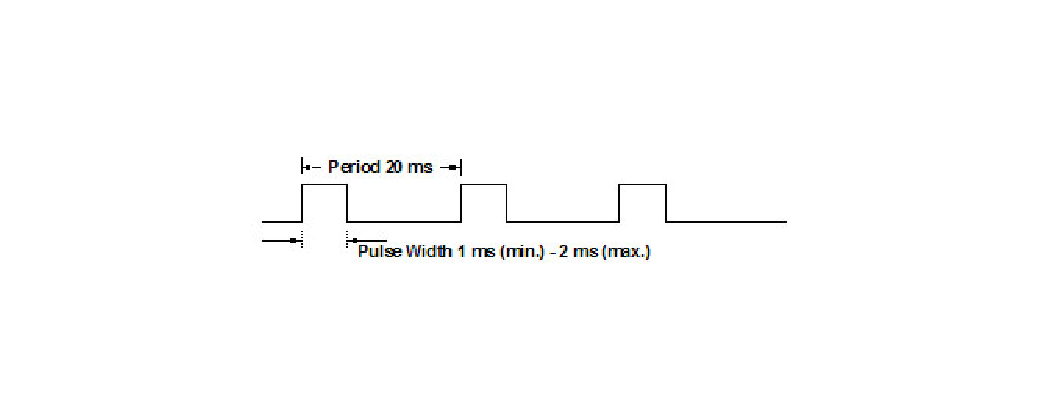
\includegraphics[width=1.0\textwidth]{figures/ServoPwm}
    \caption{\label{ServoPwm}Sch\'ema de la modulation du signal
      \'electrique \protect
      \cite{WikiServo}
    }
\end{figure}

Comme l'on peut voir, le dit signal, est form\'e de hauts et de
bas. Lorsqu'il est ``bas'', cela veut dire que la tension est basse ou \'egale
\`a 0V. Lorsqu'il est
``haut'', cela veut dire que la tension est a une valeure d\'efinie auparavant,
standard, diff\'erente de 0V. Dans notre cas, le ``haut'' est \`a 5V (standard
pour le mod\'elisme et l'\'electronique en g\'en\'eral). On appelle la
p\'eriode pendant laquelle le signal est ``haut'' une pulsation.

Chaque d\'ebut de pulsation est s\'epar\'e par un temp bien d\'efini de
20ms. Ce qui peut varier d'une pulsation \`a l'autre, donc ce qui informe le
servo en quel angle il doit se positionner, est la longueur de la
pulsation. Comme indiqu\'e, celle-ci peut varier de 1ms \`a 2ms.

\subsection{Programmation pour contr\^oler un servo}
Le programme suivant est un exemple propos\'e dans la section
``apprentissage'' du site officiel d'Arduino. Il utilise la librairie
``Servo'' install\'ee avec l'IDE Arduino. Ce que font les m\'ethodes de cette
classe est de produire un signal comme celui discut\'e \`a la section
pr\'ec\'edente et l'\'emettre par le pin choisi.

Les commentaires sont en anglais, mais le code sera expliqu\'e tout de suite:

\lstinputlisting[language=Java]{code/ServoExample.java}

\textbf{Commentaires:}

On commence par inclure la classe Servo, puis on cr\'ee un objet
\emph{Servo}. Dans la fonction \emph{setup} du programme, on lie l'objet
\emph{myservo} au pin 9 de l'arduino. Ensuite, dans la fonction \emph{loop}, on
fait varier la position du servo gr\^ace \`a la m\'ethode \emph{write}. Un
d\'elai (le programme s'arr\^ete en ce point) de 15ms pour permettre au servo
d'atteindre la position demand\'ee. Etant donn\'e que cette op\'eration est
itt\'er\'ee plusieurs fois au moyen d'une boucle \emph{for}, on pourra voir le
servo d\'ecrire un mouvement de balayage.

D'ailleur, ce programme est tr\`es pratique pour tester le fonctionement d'un servo. 

\section{Moteur de propulsion}

\subsection{Descriptif}

Le moteur de propulsion, au contraire du servo, n'a pas été changé.
 Ses caract\'eristiques \'electriques (donn\'ees que nous avon mesur\'e \`a l'aide
d'un multim\`etre du gymnase) se trouvent \`a la section
(\ref{TableDesc}). Le moteur est muni d'une boite \`a vitesse ainsi qu'un
diff\'erentiel. Nous avons estim\'e qu'il aurait \'et\'e
inutilement compliqu\'e d'y apporter des modifications. La
configuration d\'ej\`a existente, \`a l'exception de l'\'electronique,
subvient tout \`a fait \`a nos besoins.  

\subsection{H-bridge}
Faire tourner l'axe d'un moteur \'electrique pose peu de probl\`emes. Il
suffit de connecter l'un des p\^oles \`a la tention positive et l'autre \`a la tension
n\'egative. Ceci fera tourner l'axe du moteur dans un sens. Si vous souhaitez le
faire tourner dans le sens inverse, il vous suffira d'\'echanger les fils
\'electriques aux p\^oles du moteur.

Le probl\`eme suivant se pose alors: comment inverser le sens de marche du
moteur sans intervention manuelle?

La r\'eponse est donn\'ee par un astucieux circuit compos\'e de
transistors. Il permet, au moyen de deux signaux actionnant les transistors,
de contr\^oler le sens du courrant passant dans le moteur.

Le sch\'ema suivant pourra d'avantage \'eclairer le lecteur:

\begin{figure}[h]
\centering
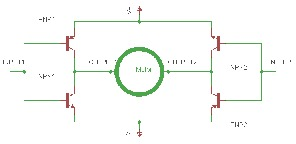
\includegraphics[width=1.0\textwidth]{figures/H-bridge}
    \caption{\label{H-bridge}Sch\'ema d'un H-bridge}
\end{figure}

\textbf{Explications:}

Tout d'abord, que sont des transistors NPN et PNP? La diff\'erence pratique
entre ces deux types de transistors est que l'un demande un signal
d\'eclencheur haut pour \^etre ouvert tandis que l'autre en demande un
bas ou la terre. Dans ce cas, on utilise deux types de transistors
diff\'erents (en grande partie pour clarifier le sch\'ema), mais l'on pourrait
tr\`es bien utiliser uniquement des transistors du m\^eme type. On obtiendrait
le m\^eme r\'esultat en connectant les \emph{INPUT} \`a des transistors
diagonalement oppos\'es\cite{RobotRoom}.

On peut voir que selon le \emph{INPUT}, on obtiendra des tensions au bornes du
moteur ou \emph{OUTPUT} variables.
\subsection{Table de V\'erit\'e}
R\'edigeons un tableau de v\'erit\'e pour mieux illustrer la situation, o\`u H
(\textit{high}) signifie haut et L (\textit{low}) signifie bas :

\begin{table}[h]
\begin{center}
  \begin{tabular}{c|c||c}  
    \emph{INPUT1} & \emph{INPUT2}
    & Tension\\
    \hline
    H & L & \emph{OUTPUT1} $=$ \emph{OUTPUT2}\\
    L & H & \emph{OUTPUT1} $=$ \emph{OUTPUT2}\\
    H & H & \emph{OUTPUT2} $>$ \emph{OUTPUT1}\\
    L & L & \emph{OUTPUT1} $>$ \emph{OUTPUT2}\\
  \end{tabular}
\end{center}

\caption{\label{tableDeVerite} Table de v\'erit\'e accompagnant le sch\'ema du
H-bridge (fig.(\ref{H-bridge}))}

Quand les signaux \emph{INPUT} sont oppos\'es, le moteur est \`a
l'arr\^et. Quand ils sont \'equivalents, le moteur est en marche, dans un sens
ou dans l'autre.

\end{table}

\subsection{L293d}
Nous avons décidé de ne pas construire notre propre H-Bridge, mais plutôt
exploiter un chip qui sert le même but. Le chip en question est dénommé
L293D. Pour commencer, une synthèse de la feuille de spécifications:

\begin{figure}[h!]
\centering
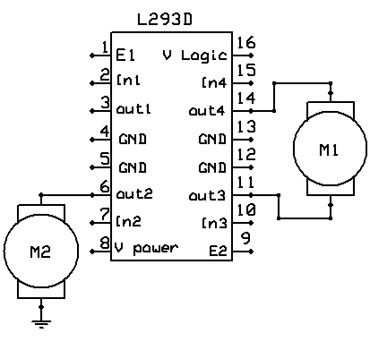
\includegraphics[width=0.5\textwidth]{figures/l293d}
    \caption{\label{l293d} Schéma du l293d.
    \protect\footnotemark}
\end{figure}
\footnotetext{http://ikalogic.cluster006.ovh.net/wp-content/uploads/l293d.jpg}

Spécifications max:

\begin{table}[h!]
\begin{center}
  \begin{tabular}{|c|c|}
    \hline
    $V_{logic}$ & $36V$\\
    \hline
    $V_{power}$ & $36V$\\
    \hline
    Peak output current & $\pm 2A$\\
    \hline
    Dissipation de chaleur à température ambiante (25°) & $2075mW$\\
    \hline
    Température max & $70°$\\
    \hline
   
  \end{tabular}
\end{center}
\caption{\label{l293dMax} Informations tirées des fiches téchniques publiées
      par TI \cite{l293dDataSheet}}
\end{table}


\subsection{Code}

Maintenant que nous avons compris le fonctionement d'un H-bridge, en
particulier les cons\'equences d'\emph{INPUT} diff\'erents, on pourra cr\'eer
un petit programme Arduino pour contr\^oler un moteur.

Le code suivant a \'et\'e r\'edig\'e par nos soins:

\lstinputlisting[language=Java]{code/motor.java}




\part{Hardware}

\section{Choix du hardware}
Pour réaliser ce projet, nous avons dû faire des choix au niveau du hardware. Notre choix s'est porté sur deux système. Le premier, l'Arduino, est un microcontrolleur qui permet de contrôler presque ce qu'on veut grâce à un language de programation proche du C. Le second est le Raspberry Pi, qui est un ordinateur bon marché (trente-cinq francs) qui est récemment sorti sur les marchés. 


\subsection{Arduino}
L'Arduino \cite{Arduino} est un microcontrolleur \textit{Open Source}, ce qui veut dire que tout le monde peut non seulement avoir accès aux plans et aux codes, mais peut aussi les modifier. Ce microcontrolleur se programme avec un language proche du C. 


\subsubsection{Choix du type d'Arduino}



\subsection{Raspberry Pi}
Le Raspberry Pi\cite{RaspberryPiCaracteristiques} est un ordinateur de la taille d'une carte de crédit sur lequel on peut installer différents systèmes d'exploitations dérivés de UNIX/Linux. Le Raspberry Pi est acheté nu, c'est-à-dire que cet ordinateur ne possède pas d'écran, ni de clavier ou de souris, néanmoins le Raspberry Pi possède plusieurs ports où on peut brancher écran (via l'interface HDMI ou Composite), un câble Ethernet et presque ce qu'on veut grâce aux deux ports USB. Le Raspberry Pi est très interressant non pas du point de vue de sa puissance calculatoire, mais du point de vue rapport qualité-prix. En effet, pour trente-cinq francs, il a les caractéristiques suivantes: 
\begin{enumerate}
\item poid de 45g environ
\item Processeur ARM1176JZF-S (ARMv6) 700MHz Broadcom 2835
\item 512Mo de RAM (sur la version B, soit celle que nous avons choisie)
\item 2 sorties vidéo (HDMI et Composite) 
\item Sortie audio stéréo Jack (3.5mm) (le son passe aussi par le HDMI en sortie 5.1)
\item Ecriture et lecture possible sur une carte mémoire sous forme de carte SD (supporte les formats: SDHC, MMC et SDIO)
\item 2 ports USB 2.0 et 1 port Ethernet
\item Alimentation par câble micro USB
\item Faible consommation (5W, 5V, 1A)
\item Communication possible via les Pin GPIO
\item Décodeur permettant de lire le FullHD  1080p
\item API logiciel vidéo (OpenGL)
\end{enumerate}
Bien qu'à première vue la Framboise ne semble pas très performante, il faut prendre en compte son prix qui est bas, sa taille ainsi que les possibilités qui sont presque infinies.

\subsubsection{Choix de l'OS}
Plusieurs types de systèmes d'exploitations fonctionnant sur le Raspberry Pi existent. Pour n'en citer que quelques-uns:
\begin{multicols}{2}
\begin{itemize}
\item Androïd
\item Firefox OS
\item RISC OS
\item Fedora
\item Debian
\item ArchLinux
\item Gentoo
\item Raspbian
\end{itemize}
\end{multicols}
Notre choix à été porté sur Raspbian, qui est un dérivé de Debian, pour plusieurs raisons. Tout d'abord, cet OS à été dévellopé spécialement pour le Raspberry Pi et il est donc continuellement dévellopé par la communauté du Raspberry Pi. Cet OS étant basé sur un environnement Linux, cela offre un grand nombre de liberté afin de travailler dessus. Raspbian est aussi gratuit, se qui rentre en compte puisque nous essayons de réduire les coûts.  


\part{Software}


\bibliographystyle{plain}
\bibliography{references}


}

\end{document}
